% =============================================================================

% Conception — Patrons de conception (catalogue GoF)

% TicketManager — formulation académique

% Prérequis document principal : \usepackage{multirow} \usepackage{float}

% Figures : docs/release-1/img/ — palette harmonisée avec les diag. de séquence

% =============================================================================



\subsection{Patrons de conception utilisés}



La conception logicielle de \textit{TicketManager} mobilise un ensemble restreint

de patrons de conception, issus des familles \textbf{création},

\textbf{structurels} et \textbf{comportementaux} (Gamma \textit{et al.}, 1994).

Le tableau~\ref{tab:catalogue-patrons} en présente la synthèse ; les

figures~\ref{fig:patron-fabrique-module} à~\ref{fig:patron-observateur} en

illustrent la structure par diagrammes de classes.



\begin{table}[H]

\centering

\footnotesize

\renewcommand{\arraystretch}{1.2}

\setlength{\tabcolsep}{6pt}

\begin{tabular}{|p{3.2cm}|p{4.2cm}|p{5.8cm}|}

\hline

\textbf{Famille} & \textbf{Patron} & \textbf{Contexte d'application} \\

\hline

Création & Fabrique (module) & Instanciation des services par domaine métier \\

\hline

Structurels & Décorateur & Enrichissement des accès par métadonnées de sécurité \\

\hline

\multirow{3}{*}{Comportementaux} & Stratégie & Mécanisme d'authentification interchangeable \\

\cline{2-3}

 & Chaîne de responsabilité & Filtrage séquentiel des requêtes entrantes \\

\cline{2-3}

 & Observateur & Notification proactive des acteurs concernés \\

\hline

\end{tabular}

\caption{Catalogue des patrons de conception — TicketManager}

\label{tab:catalogue-patrons}

\end{table}





% ---------------------------------------------------------------------------

\subsubsection{Patron de création — Fabrique (module)}

% ---------------------------------------------------------------------------



Chaque domaine fonctionnel (authentification, utilisateurs, tickets,

notifications) est encapsulé dans un module dédié qui centralise la

déclaration et l'instanciation de ses composants. Ce mécanisme de fabrique

logique garantit une frontière claire entre les espaces métier.



\begin{figure}[htbp]

    \centering

    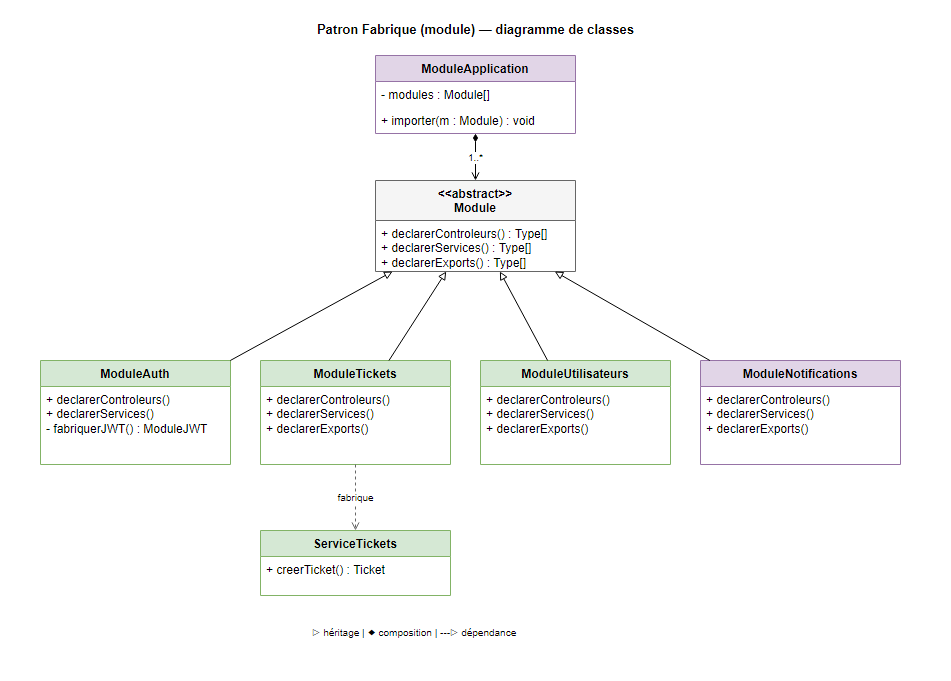
\includegraphics[width=0.88\textwidth]{img/patron-fabrique-module.png}

    \caption{Patron Fabrique (module) — diagramme de classes}

    \label{fig:patron-fabrique-module}

\end{figure}





% ---------------------------------------------------------------------------

\subsubsection{Patron structurel — Décorateur}

% ---------------------------------------------------------------------------



Certaines opérations sont annotées de métadonnées de sécurité (rôle requis,

accès public autorisé) qui modifient dynamiquement le comportement du

traitement sans altérer la structure du contrôleur sous-jacent.



\begin{figure}[htbp]

    \centering

    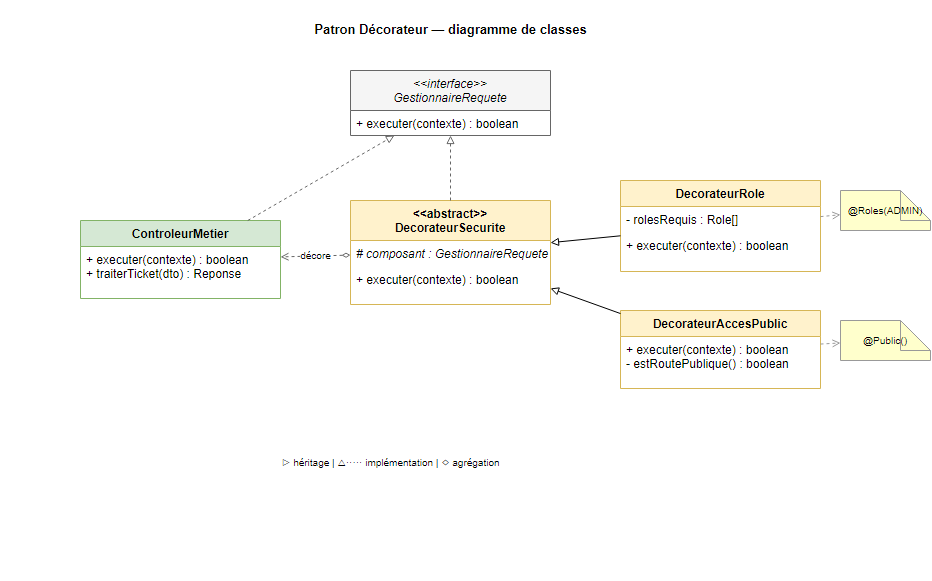
\includegraphics[width=0.85\textwidth]{img/patron-decorateur.png}

    \caption{Patron Décorateur — diagramme de classes}

    \label{fig:patron-decorateur}

\end{figure}





% ---------------------------------------------------------------------------

\subsubsection{Patrons comportementaux}

% ---------------------------------------------------------------------------



\paragraph{Stratégie.}

L'authentification repose sur une stratégie de validation des identifiants

interchangeable : le mécanisme de vérification du jeton d'accès peut être

substitué sans remettre en cause le reste de l'application.



\begin{figure}[htbp]

    \centering

    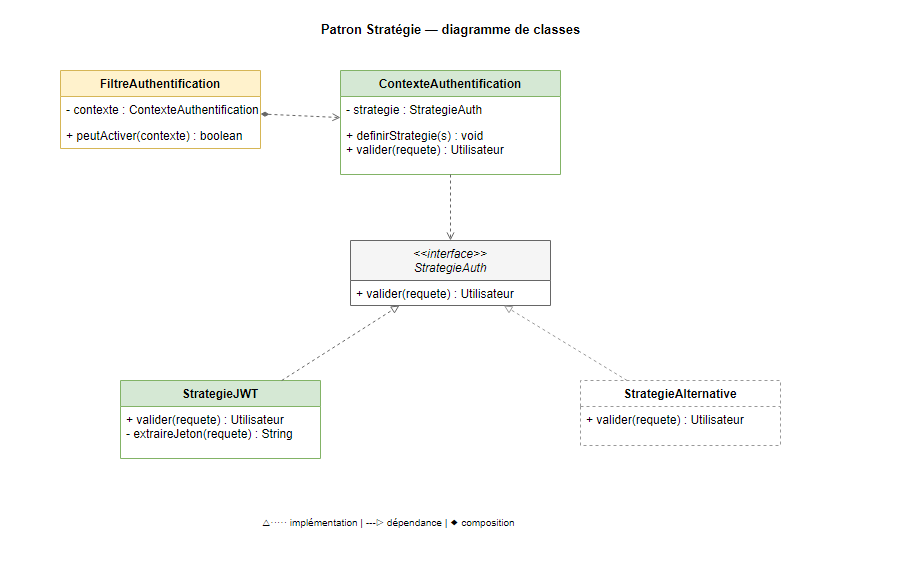
\includegraphics[width=0.85\textwidth]{img/patron-strategie.png}

    \caption{Patron Stratégie — diagramme de classes}

    \label{fig:patron-strategie}

\end{figure}



\paragraph{Chaîne de responsabilité.}

Chaque requête entrante traverse une succession de filtres de sécurité :

identification de l'utilisateur, contrôle de son profil, vérification de ses

droits sur la ressource visée. En cas d'échec, la requête est rejetée avant

d'atteindre la logique métier.



\begin{figure}[htbp]

    \centering

    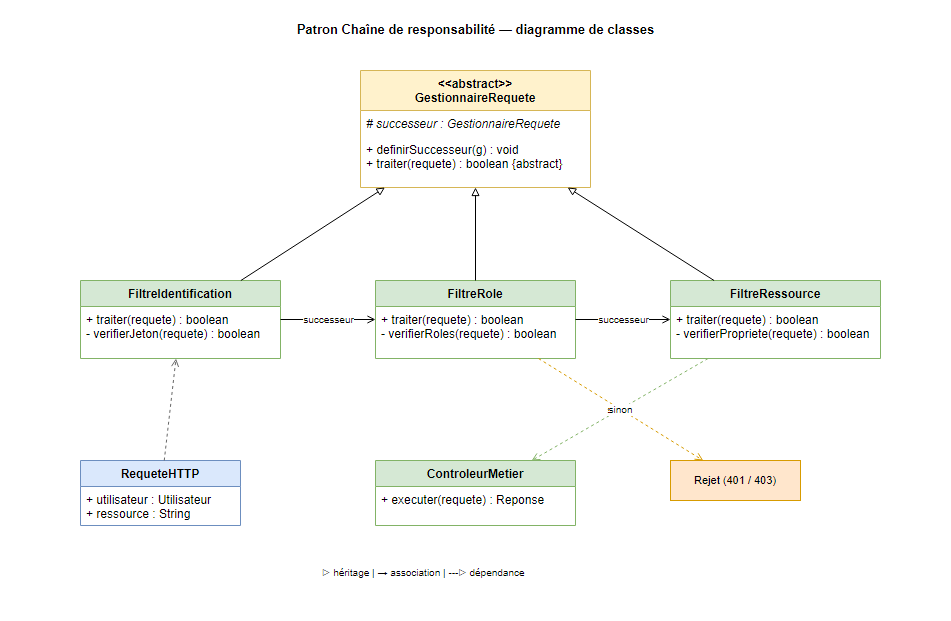
\includegraphics[width=0.88\textwidth]{img/patron-chaine-responsabilite.png}

    \caption{Patron Chaîne de responsabilité — diagramme de classes}

    \label{fig:patron-chaine-responsabilite}

\end{figure}



\paragraph{Observateur.}

Lorsqu'un événement significatif survient sur un ticket (création, assignation,

changement de statut), le système notifie de manière proactive les acteurs

concernés, sans que ceux-ci aient à interroger périodiquement le serveur.



\begin{figure}[htbp]

    \centering

    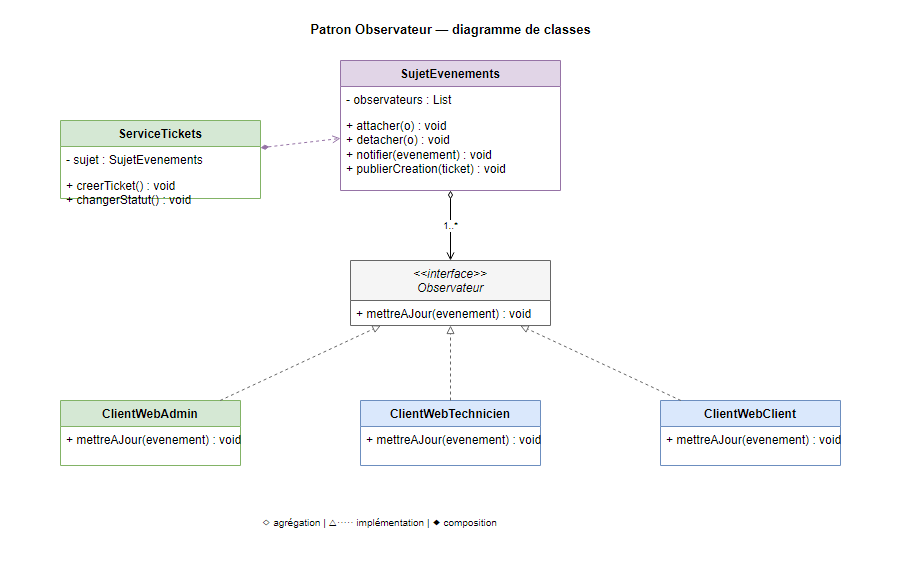
\includegraphics[width=0.88\textwidth]{img/patron-observateur.png}

    \caption{Patron Observateur — diagramme de classes}

    \label{fig:patron-observateur}

\end{figure}


